\newbox\mybox
{
  \parindent0pt
  \null
  \definecolor{color2}{HTML}{b45412}
  \definecolor{color3}{HTML}{b45412}
  \newfontface\titleface[Scale=4]{Arial}
  \thispagestyle{empty}
  \vfill
  \hfil
  \begin{tikzpicture}[overlay]
    \coordinate (left) at (-.55\paperwidth,0);
    \coordinate (right) at (0.55\paperwidth,0);
    \coordinate (top) at (0,.55\paperheight);
    \coordinate (bottom) at (0,-0.55\paperheight);
    \coordinate (bandstart) at (0,0.15\paperheight);
    \coordinate (bandend) at (0,0.2\paperheight);
    \fill [black!02] (bottom -|left) rectangle (top-|right);
    \draw (-10mm,80mm) node
    {\titleface \textcolor{color3}{
          macroeconomics}};
    \fill [color2] (bandstart -|left) rectangle (bandend -| right);
    \draw (bandstart -|left) node  [xshift = 110mm,yshift=17pt] {\huge
      \textcolor{white}{\textsf{Jyotirmoy Bhattacharya}}};
    \draw (bandstart -|right) node [xshift =
    -25mm,yshift=-10pt]{\small \textcolor{color2}{\textbf{\myversion}}};
    \draw (bottom -|left) node [above right,xshift=0.1\paperwidth,yshift=15mm] {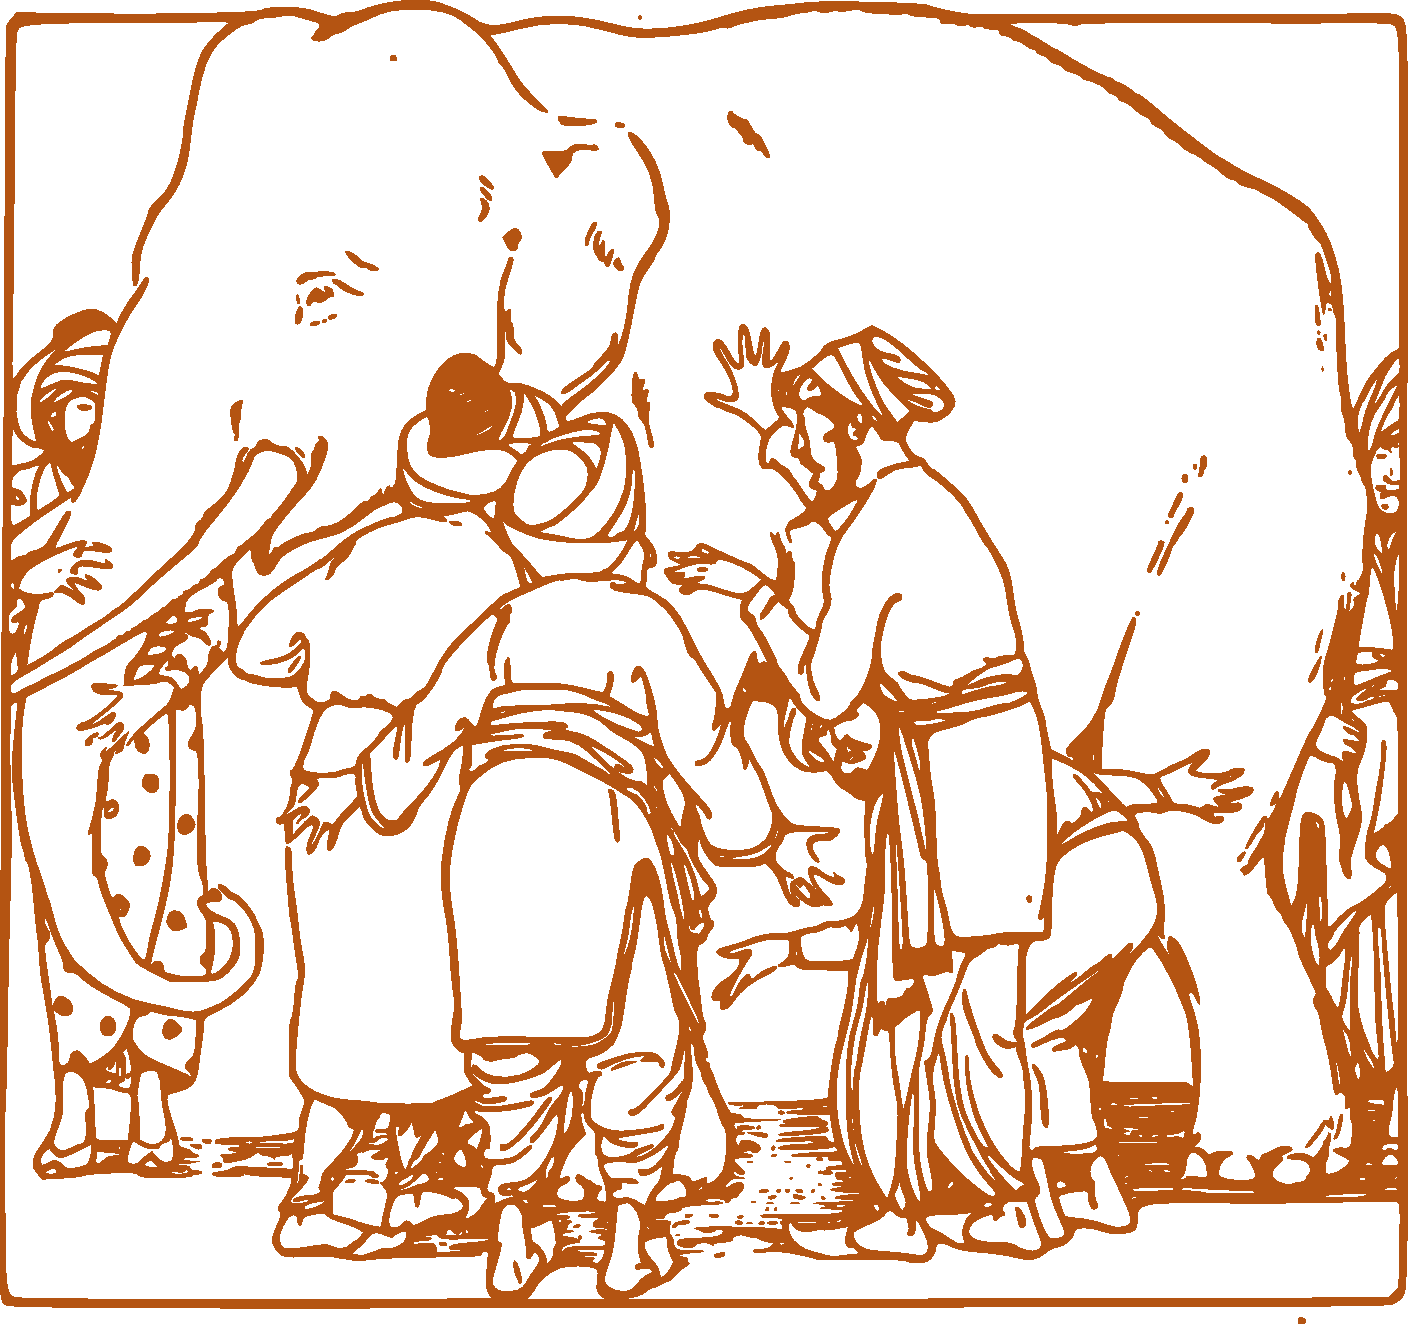
\includegraphics[width=0.8\paperwidth]{Blind_men_and_elephant.pdf}};

 %    \coordinate (front) at (0,0);
%     \coordinate (horizon) at (0,.31\paperheight);
%     \coordinate (bottom) at (0,-.6\paperheight);
%     \coordinate (sky) at (0,.57\paperheight);
%     \coordinate (left) at (-.51\paperwidth,0);
%     \coordinate (right) at (.51\paperwidth,0);

%     \shade [bottom color=blue!30!black!10,top color=blue!30!black!50]
%       ([yshift=-5mm]horizon -|  left) rectangle (sky -| right);
%     \fill [black!25] (bottom -| left) rectangle ([yshift=-5mm]front -| right);
% 
\end{tikzpicture}
\vfill
\vbox{}
\clearpage
}
